
%% 
%% Copyright 2007-2020 Elsevier Ltd
%% 
%% This file is part of the 'Elsarticle Bundle'.
%% ---------------------------------------------
%\documentclass[preprint,12pt]{elsarticle}
% \documentclass[review,12pt, 3p, times]{elsarticle}
\documentclass[preprint,11pt,3p]{elsarticle}

\usepackage{amssymb}
\usepackage{graphicx}
\usepackage{longtable}
\usepackage{tipa}
\usepackage{cancel}
\usepackage{ulem}
\usepackage{pgf}
\usepackage{silence}
\usepackage{amssymb}
\usepackage{lineno}
\usepackage{enumitem}
\usepackage{lineno,hyperref}
\usepackage{natbib,stfloats}
\usepackage{multirow}
\usepackage{array}
\usepackage{multicol}
\usepackage{booktabs}
\usepackage{mathrsfs}
\usepackage{graphicx}
\usepackage{epstopdf}
\usepackage{latexsym}
\usepackage{mathtools}
\usepackage{algorithm}
\usepackage{algorithmic}
\usepackage{amsmath,amsfonts,amssymb}
\usepackage{rotating}
\usepackage{color}
\usepackage{colortbl}
\usepackage[caption=false]{subfig}
\usepackage[ruled,vlined,algo2e]{algorithm2e}
\usepackage{setspace}
\usepackage{tabularx}
\usepackage{xcolor}
\usepackage{adjustbox}
\usepackage{tikz}

\usepackage{cancel}
\hypersetup{colorlinks,linkcolor={blue},citecolor={blue},urlcolor={red}} 

\usepackage{setspace}
\usepackage{lineno}
\usepackage{amssymb}
\usepackage{pifont}
\usepackage{svg}
\usepackage{tikz,lipsum,lmodern}
\usepackage[most]{tcolorbox}
\usepackage{pdfpages}
\usepackage{geometry}
\geometry{top=1.5cm,bottom=2.5cm,left=1.5cm,right=1.5cm}
% \definecolor{my-blue}{cmyk}{0.80, 0.13, 0.14, 0.04, 1.00}
\definecolor{q_color1}{HTML}{F0F8FF}
\definecolor{q_color2}{HTML}{91A3B0}

\definecolor{r_color1}{HTML}{d9dbde}
\definecolor{r_color2}{HTML}{737475}

\newcounter{magicrownumbers}
\newcommand\rownumber{\stepcounter{magicrownumbers}\arabic{magicrownumbers}}
\newcommand{\cmark}{\ding{51}}%
\newcommand{\xmark}{\ding{55}}%


\journal{journal of Computers and Industrial Engineering}

\begin{document}
\begin{center}
       \begin{huge}  
              \textbf{ \quad \quad Response to reviewers}
       \end{huge}  
       \newline
       \newline
       \textbf{Ms. Ref. No.: PROECO-D-23-01945}
                     
       \textbf{Title: "Incorporating Uncertain Human Behaviour in Production Scheduling for Enhanced Productivity in Industry 5.0 context" } 
 \newline
 International Journal of Production Economics 
       
\end{center}

First, we thank all the reviewers for the thorough revision and valuable comments on the previous version. We have carefully read and analyzed each of your comments and considered them in preparing this new version. We hope that this new version is now much clearer. The following explains our interpretation of your comments and how we considered each. In addition, the paragraphs containing modifications have been highlighted in the text (in blue). We have also linked each comment to the corresponding point in the manuscript using the notation "$[id]R{q}$",  "q" represents the comment number, and "id" is the comment identifier. 





\newpage 
% Thank you for the relevant remark, 


\section{Reviewer 01}
Thank you for taking the time to provide detailed feedback on our manuscript. We sincerely appreciate your thorough review and insightful comments. Your constructive criticism and valuable suggestions will undoubtedly enhance our work's quality and clarity. We have carefully considered each of your points and would like to address them accordingly.


\begin{tcolorbox}[colback=q_color1,colframe=q_color2,title=Q1:] 
The article is fairly written, the goal is clear, but some doubts arise about the 'human behaviour' concept, description of parameters employed, and the methodology used.
I suggest authors to separate introduction from literature review to highlight the novelty of the paper (i.e., I expect introduction to contain the motivation that brought authors to develop this research and the structure of the paper, then, literature review can collect the prior works and define the main novelty of this paper compared to the others). Please, consider separating the two sections to provide a solid scientific structure to this work. Moreover, a literature review section allows authors to explicit the keyworks research adopted for their work and the databases mainly investigated.
\end{tcolorbox}

\begin{tcolorbox}[colback=r_color1, colframe=r_color2, title=R1:]
We thank you for this advice which has improved the manuscript's structure and coherence. We have divided the introduction into two sections (Introduction and Literature Review) and explicitly included our method of bibliographic research at the beginning of the literature review section.   
 \end{tcolorbox}
\begin{tcolorbox}[colback=q_color1, colframe=q_color2,title=Q2:] Page 10: Are machines another agent of this problem, or are machines considered as predictable agents? According to this hypothesis, they will never break, hence, they do not have any uptime or downtime (except for the setup time) and they are not a source of unpredictability.
\end{tcolorbox}

\begin{tcolorbox}[colback=r_color1,colframe=r_color2,title=R2:]
A machine or workstation is a type of agent zone that is a predictable agent activated only when the operator is present. We explained that on page 11, where the agent zone is defined as follows: ``Zone: This agent is a reactive agent representing workstations (WS) and non-productive zones (NPZ) located in the workshop". As we focus on the operator profiles, we assume that they are performing the production operation when they are on their workstation. To avoid confusion, we use the word ``workstation" when referring to the productive zone, encompassing the production tools and the worker's workspace. 
\end{tcolorbox}

\begin{tcolorbox}[colback=q_color1,colframe=q_color2,title=Q3:] Page 12: I suggest authors to avoid the adoption of the third person such as "… and that he can only move back and forth …". I suggest authors to use "they" instead and always refer to workers, or operators.
\end{tcolorbox}

\begin{tcolorbox}[colback=r_color1,colframe=r_color2,title=R3:]
Thank you for your suggestion. We have corrected the sentences and applied the change throughout the text.
\end{tcolorbox}
\begin{tcolorbox}[colback=q_color1,colframe=q_color2,title=Q4:] Page 13: In my opinion, there is a strong hypothesis in this context: The operators are free to move to a NPZ anytime they want, according to a certain probability. This is not always true in industrial context. They surely have some breaks; Breaks can last a little longer, sometimes they have physiological need, but not always they can move freely. Authors should consider somehow that the workforce needs to stay productive until certain productivity is reached. Otherwise, there might be some issues for workers that do not comply with the productivity level the company is expecting from them if not properly justified (e.g., injuries during work activity). Did authors consider the minimum productivity in the definition of the maximum value of non-productive time?
\end{tcolorbox}

\begin{tcolorbox}[colback=r_color1,colframe=r_color2,title=R4:]
Thank you for your relevant question, which affords us the opportunity to provide more clarification concerning the context of Industry 5.0, which is a human-centered paradigm aiming to put technology and organizational structures at the service of humans. 
This paradigm gives priority to human-centered approaches aimed at aligning technology and organizational structures to meet human needs. In this context, providing operators with workstations that are adapted to their needs becomes crucial to maintaining employee motivation and productivity. In fact, productivity no longer depends solely on the presence of workers at their workstations. Unlike traditional production systems, in which workers can feel constrained and lack autonomy, Industry 5.0 seeks to give them greater freedom. This encourages motivation, creativity, and, ultimately, improved productivity while reducing turnover rates in the industrial sector, particularly in Europe. 
\end{tcolorbox}

\begin{tcolorbox}[colback=q_color1,colframe=q_color2, title=Q5:] Page 14: Authors state that "During this process, the worker is not present all the time on his workstation". Does it mean that workers do not need to stay at their workplace while machine is running? Hence, non-productive time not always impacts the productivity of workers, is it correct? Additionally, while small break and lunch break can vary in duration, the number of time that a worker goes to the nursery is not always linked to the behavior of workers, maybe it is much more related to the type of injury, the frequency and the attitude of workers to get injured on the workplace.
\end{tcolorbox}

\begin{tcolorbox}[colback=r_color1,colframe=r_color2,title=R5:]
This sentence means the worker is not obliged to stay at the workstation. However, we assume that the workstation ceases to produce when the worker leaves the productive zone. We've added more explanation on the definition of the production zone and a sentence to clarify this situation. 

We agree with your analysis that the probability of an injury can be related to the worker's experience because it is directly related to attitude and respect for safety rules. Regarding severity, it is more related to the manner of working and the manner of using the production tools. There is also a big part of hazardous events that affect the severity of the injury. The length of the stay in the nursery is linked to the severity of the injury and the worker's psychological situation, both of which are considered to be part of the worker's behavior.  

%However, it may be that two workers behave in the same way ,and one of them is injured, and the source is the work environment, which doesn't always happen. That's why we chose a probabilistic model.
%This is just one example of the link between behavior and nursing.
%In future work, we intend to dissociate (injuries and their severity) and worker behavior and add more details.

\end{tcolorbox}
\begin{tcolorbox}[colback=q_color1,colframe=q_color2,title=Q6  :] Page 16: I believe the assumption "Each machine is assigned only one worker" is redundant with constraint 3 and 4, saying that "Constraints (3) and (4) ensure that each machine is assigned to one worker and that each worker is assigned to at most one machine".
\end{tcolorbox}

\begin{tcolorbox}[colback=r_color1,colframe=r_color2,title=R6:]
Thank you for your comment. Indeed, constraints 3 and 4 represent the formulation of assumption 3. We have included a sentence to clarify that they are provided in accordance with assumption 3.

\end{tcolorbox}
\begin{tcolorbox}[colback=q_color1,colframe=q_color2,title=Q7  :] There are some typos in the text, such as on page 19: "Constraints (6) ensures that the minimum production mix is respected. Constraints (7) ensures a strict production sequence …" I suggest the author consider an English proofreading of this manuscript before its resubmission. Lots of typos can disrupt the quality of the work. Hence, I am confident that the University can help authors professionally proofread this manuscript before resubmission.
\end{tcolorbox}

\begin{tcolorbox}[colback=r_color1,colframe=r_color2,title=R7:]
All the English of the paper has been revised.
\end{tcolorbox}
\begin{tcolorbox}[colback=q_color1,colframe=q_color2,title=Q8  :] Figure 5 is still very difficult to follow. I suggest authors to dedicate more space to the layout of this figure and provide some more explanation of each part of the flowchart.
\end{tcolorbox}

\begin{tcolorbox}[colback=r_color1,colframe=r_color2,title=R8:]
Effectively Figure 5 was not well explained. We added a paragraph to explain the computation process illustrated by this figure. 
\end{tcolorbox}
\begin{tcolorbox}[colback=q_color1,colframe=q_color2,title=Q9:] Following the assumption "Once a worker is assigned to a machine, their assignment remains unchanged throughout the entire scheduling period", Figure 6 shows that three workers are assigned to machines 1, 2, and 3; however, this means that two workers are not assigned to any machines until the end of the turn, is it correct?
\end{tcolorbox}

\begin{tcolorbox}[colback=r_color1,colframe=r_color2,title=R9:]
Yes, that is absolutely true. During one planning period, our objective is to maximize productivity with the available team. However, in another planning period, we might have a different team of workers with a different mix of behaviors. This scenario can result in situations where the same operator could be assigned to a different workstation.

\end{tcolorbox}

\begin{tcolorbox}[colback=q_color1,colframe=q_color2,title=Q10:] 
Following my previous comment, is this exclusion only a matter of skills needed to work (especially) on bottleneck machines, or does the excluded workers are the ones with less productivity and less attitude to continuously work? In such a way, workers may perceive they are discriminated from an equal selection, and this may lower workers' morale. The algorithm always looks for the best solution (i.e., lower makespan or higher productivity) excluding the operators with less proneness to work in such a context. This may bring to some legal issues for company that, by applying this algorithm, can ask to the same people to work on the machines based on their skills. How do authors want to address such issue in a moment where social sustainability and workforce inclusion are such sensible themes?
\end{tcolorbox}

\begin{tcolorbox}[colback=r_color1,colframe=r_color2,title=R10:]
Thank you for this remark. We think that the algorithm deals with an operational decision that aims to maximize productivity. However, considering inclusion and skill development of workers is a part of the tactical decision that can be ensured with the rotation of teams and the variability of the production mix. We think that the algorithm can provide a more inclusive situation where persons with non-adaptive profiles at a workstation will be automatically assigned to another workstation where they can keep their place and continue contributing to the production. We added more discussion on this point in the managerial insights. % on doit rajouter quelque chose dans le mangeria insignte qui montre queue notre algorithm augmented l'nclusivité des operateurs. 
\end{tcolorbox}

\begin{tcolorbox}[colback=q_color1,colframe=q_color2,title=Q11  :] Page 22: Please, consider not to use the short form of sentence such as "Although the observation of the use case doesn't allow for …"; authors may prefer to use "does not" instead.
\end{tcolorbox}

\begin{tcolorbox}[colback=r_color1,colframe=r_color2,title=R11:]
All the English of the paper have been checked. 
\end{tcolorbox}
\begin{tcolorbox}[colback=q_color1,colframe=q_color2,title=Q12  :] Page 24: I would like to raise a discussion on nursery as a NPZ: Is the non-productive time spent in infirmary for care imputable to worker's behavior, or is it a duration that can also depend from the gravity of the injuries the workers and not from the individual behavior?
\end{tcolorbox}

\begin{tcolorbox}[colback=r_color1,colframe=r_color2,title=R12:]
%We understand that the duration and frequency of visiting the NPZ nursery are influenced not only by factors related to worker personality, but also by others related to the uncertain context, even its influence could be supposed less than the individual personality of the worker. 
%We added a paragraph about the NPZ nursery to explain and justify better our assumption regarding this aspect. 
We understand that the duration and frequency of visiting the NPZ nursery are influenced not only by factors related to worker personality but also by others related to the uncertain context, even though its influence could be considered less than that of personality. Moreover, stochastic modelling makes it possible to aggregate the influences of the two sources of variation. We added a paragraph about the NPZ nursery to explain and justify better our assumption regarding this aspect. 

%the stochastic modelling of the behaviour include the tow component wWhile we have identified a behavior, it is not the sole determining factor the actions that operate is conducing. Therefore, we model the characteristics of these actions using a stochastic parameter. We added a paragraph about the nursery's non-productive zone to explain that.

% In fact, we agree with you that the time spent in the infirmary is positively correlated with the gravity of the injuries. However, we assume that the frequency and the gravity of injuries are mostly dependent on the individual behavior (compliance with safety rules, seniority, etc.)
\end{tcolorbox}
\begin{tcolorbox}[colback=q_color1,colframe=q_color2,title=Q13  :] Page 26: I suggest authors to take one scenario as an example (e.g., such as the C31 as an example) to provide more detail and explain the meaning and the impact that the sequence (5,0,0,0,0,0) has on the productivity. Moreover, are the process time clearly stated in this numerical example to let the reader eventually replicate the numerical test?
\end{tcolorbox}

\begin{tcolorbox}[colback=r_color1,colframe=r_color2,title=R13:]
Thank you once more for your feedback. We have incorporated an illustrative example and ensured that all parameters used are clearly defined, allowing readers to replicate the test.
\end{tcolorbox}
\begin{tcolorbox}[colback=q_color1,colframe=q_color2,title=Q14  :] Page 28: Since the model is not linear, which is the computation time to find the optimal solution? Did author consider using a heuristic to solve the problem in case of greater number of jobs?
\end{tcolorbox}

\begin{tcolorbox}[colback=r_color1,colframe=r_color2,title=R14:]
For the majority of tested instances, with one product type and one week time horizon, the solver takes around 13 minutes in average.  We add the computation time in all tables of results. For one week of time horizon, it seems not needed to develop a specific heuristic to educe resolution time, however it can be interesting to test some meta-heuristics to test their performances or to include other objectives.  
In terms of computation time, we have re-executed all test experiments using a new computer with enhanced capabilities: an Intel(R) Core(TM) i9-14900HX 2.20 GHz CPU with a 2.40 GHz processor and 32.0 GB of RAM. This enables us to resolve scenarios involving multi-product and multi-profile (group (GH)) of a one-week time horizon in a reasonable computation time (13 to 14 minutes).
% The model contains two 
% In addition, the computation time generally increases with the profile mix and product mix, where the computation time in global scenarios with a horizon of one day (8 hours) jump from [XXX] minutes , but it increases to [XXX] minutes with a highest mix of profiles (a worker from each profile [1,1,1,1,1,1] in the scenario group GH). It increases also with number of product types, where it takes [XXX] hours with 1 product types and [XXX] with three product types. for a horizon of one week, it cannot resolve the problem in less then 24 hour with the worst scenario (a worker from each profile and a product from each type). 
% As this computation time increases with the planning horizon and profile mix heterogeneity, we are working on the development of a meta-heuristic to solve larger instances.

% On page 41 "In the next step, we plan to improve our human behavior models by incorporating factors such as experience, skills, and personality to improve the accuracy of the proposed optimization model. Moreover, it will be worthwhile to develop approximate methods (e.g., metaheuristics) to solve the proposed optimization model." 
\end{tcolorbox}

\begin{tcolorbox}[colback=q_color1,colframe=q_color2,title=Q15  :] One of the main conclusions the authors report in the discussion is the following: "The optimal allocation strategy involves assigning the best available profiles to the bottleneck workstation with the longest processing time," which is quite predictable as a result.suggest that the authors focus more on the heterogeneity of the workers to provide some interesting insights to the management.The company needs to deal with heterogeneous workers and high turnover continuously; however,workers who do not have enough skills cannot be put aside since they can actively contribute to the final throughput of the day. Which are the suggestions the authors want to leave to the company to manage workers' heterogeneity better?
\end{tcolorbox}

\begin{tcolorbox}[colback=r_color1,colframe=r_color2,title=R15:]
We appreciate your feedback and your suggestions regarding the heterogeneity of profiles and their impact on production. 
Therefore, we have included additional analyses on this topic in the paper on pages 39-41. These analyses provide a more comprehensive understanding of the relationship between profile heterogeneity and production outcomes. We also added some discussions to understand better the relationship between worker heterogeneity, worker skills and turnover.
This solution enables the use of all available profiles, considering current levels of skills and motivations. The ability to test various scenarios representing different combinations of profiles provides an exciting tool for human resources managers to define their strategies for shits/crew planning, recruiting, training, and skills enhancement.
\end{tcolorbox}

\begin{tcolorbox}[colback=q_color1,colframe=q_color2,title=Q16  :] Page 38: Which is the maximum dimension of the scenario that the solver of the MINLP can manage before the simulation results becomes more valuable in terms of computational time and complexity? Did authors think already to a heuristic or meta-heuristic approach that can take place of the solver for the MINLP in case of big scenario?
\end{tcolorbox}
% \begin{figure}
%     \centering
%     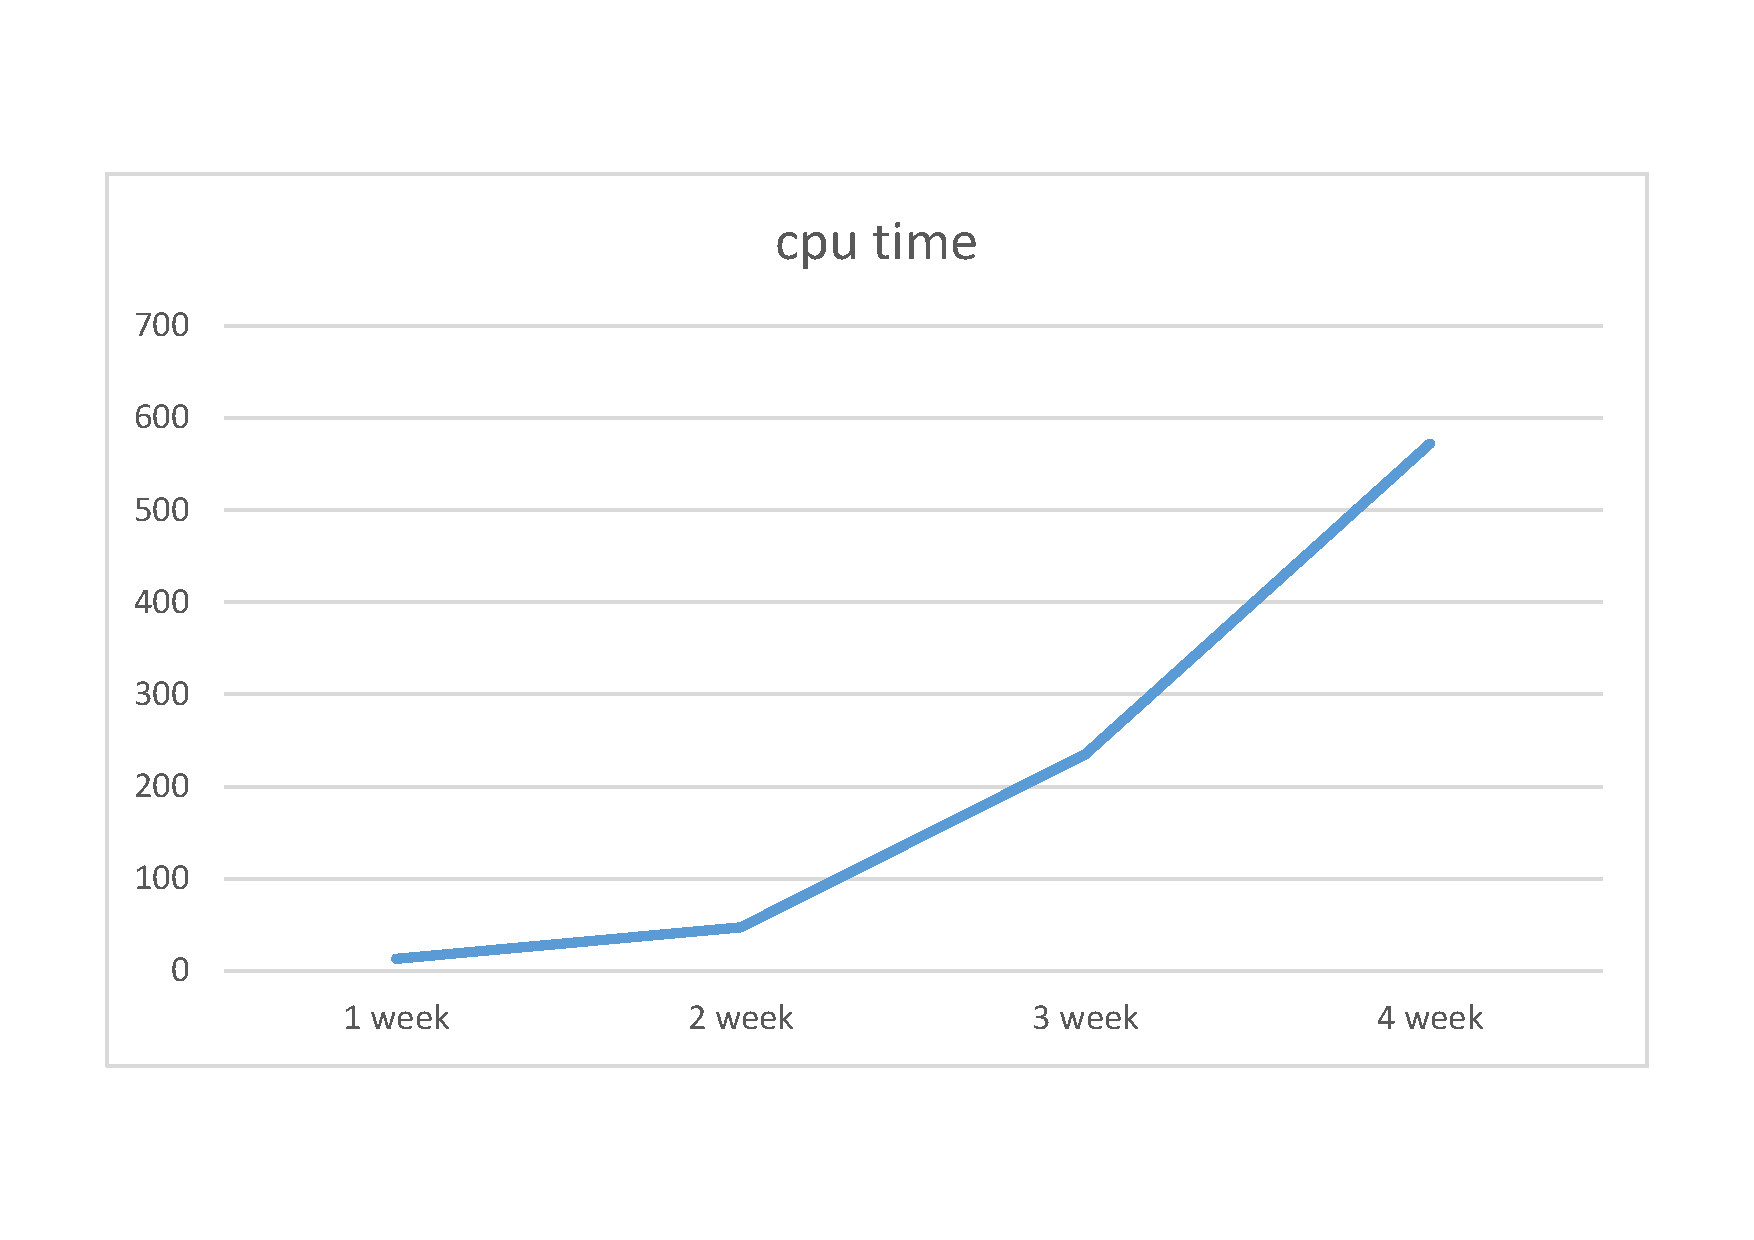
\includegraphics[trim=0 55 0 30,clip,width=15cm]{cpu time.pdf}
%     \label{fig:enter-label}
% \end{figure}
\begin{tcolorbox}[colback=r_color1,colframe=r_color2,title=R16:]
The most complex case, with a total mix of products (3 types) and a total mix of worker profiles (6 profiles), takes around 13 minutes for a time horizon of one day and more than 4 hours for a time horizon of 3 weeks (see figure below).
% we stopped the sovler after two days of computation. This why we reduced the horizon to one plannification day that can be solved in average of XXX minutes. 
% over 600 jobs, the solver starts to give a solution over a long period. 
We note that 
That's why we've proposed a heuristic or meta-heuristic approach for future work on page 41.\\
\begin{center}
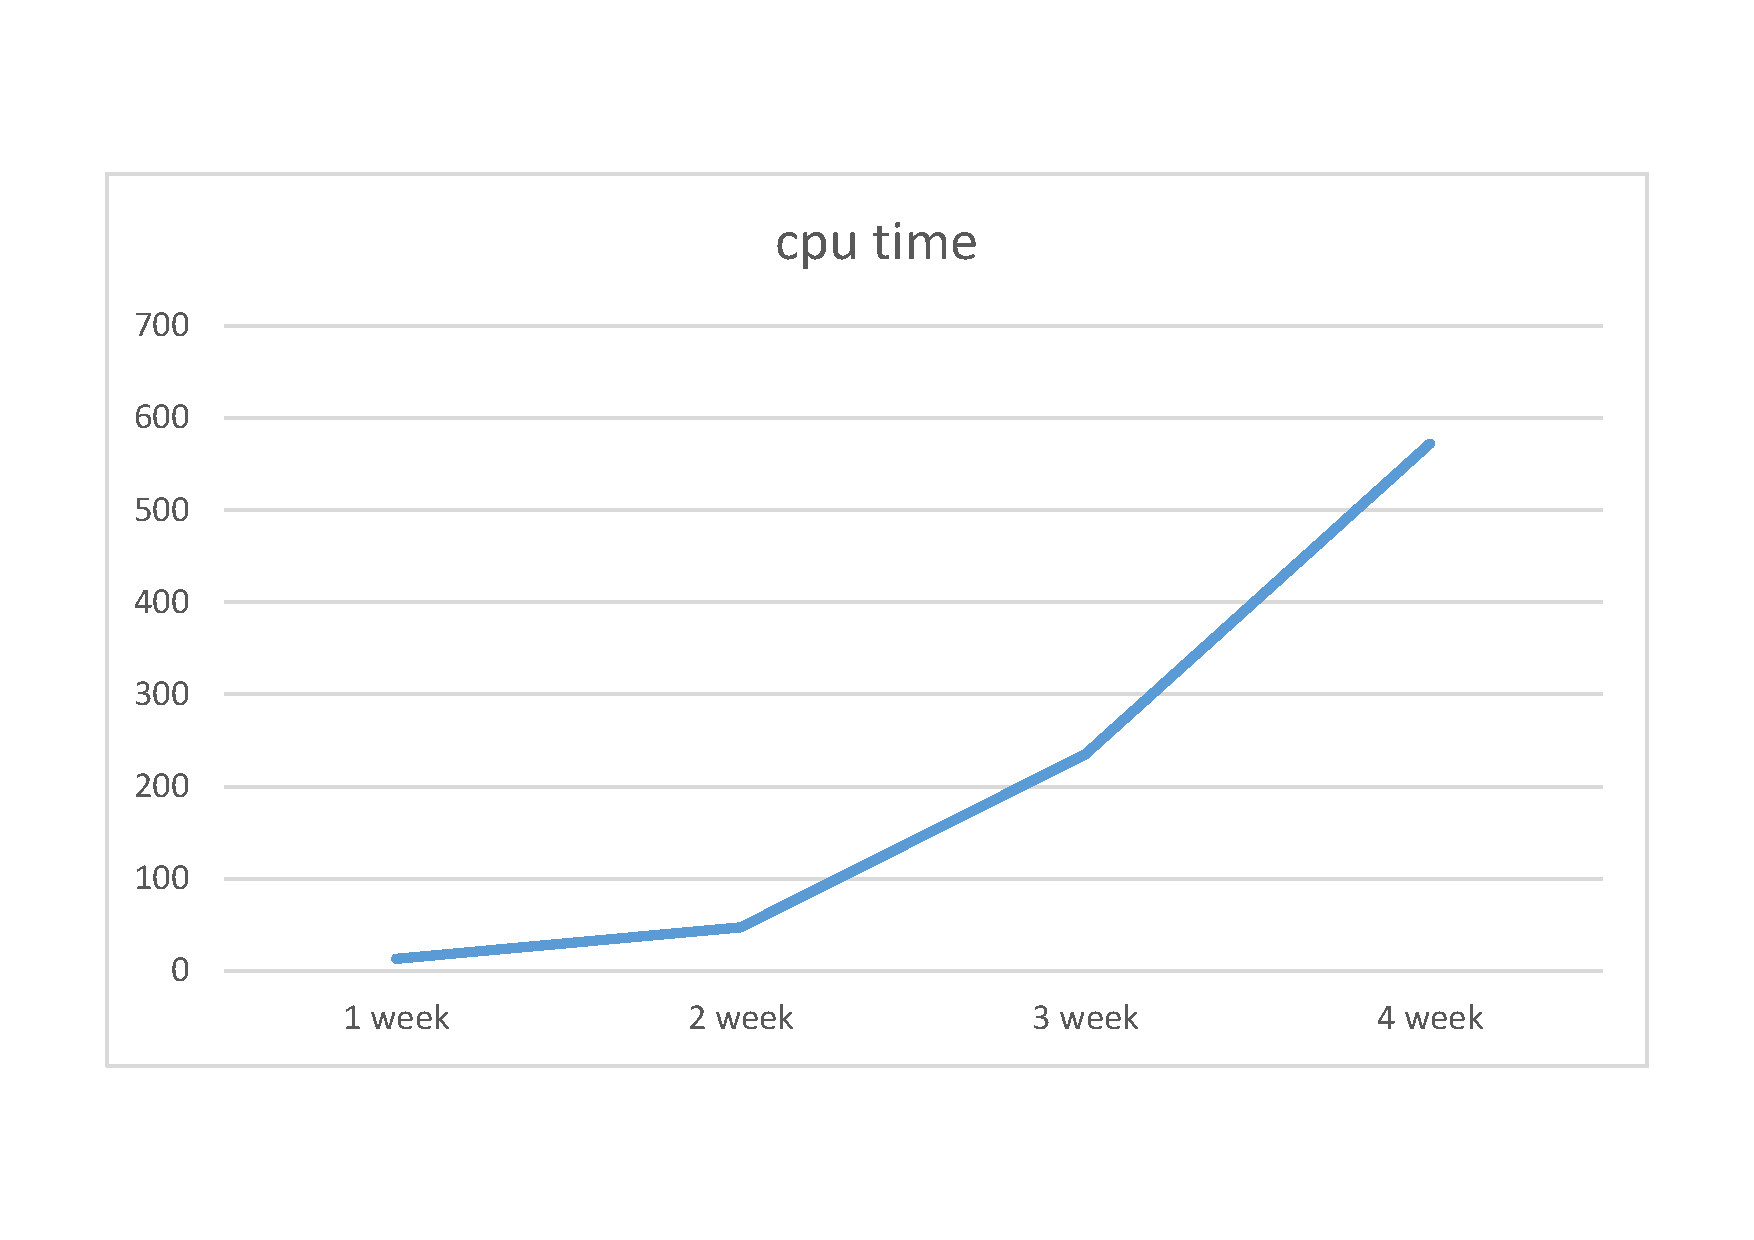
\includegraphics[trim=0 55 0 30,clip,width=10cm]{cpu time.pdf} 
\end{center}
\end{tcolorbox}
\begin{tcolorbox}[colback=q_color1,colframe=q_color2,title=Q17  :] Please carefully check the references of this work, some have been doubled and some others have been miswritten during the review process, compared to the original work.
\end{tcolorbox}

\begin{tcolorbox}[colback=r_color1,colframe=r_color2,title=R17:]
% battini2022towards  ; Battini2022
Thank your for your rigor. This issue has been corrected.
\end{tcolorbox}
\begin{tcolorbox}[colback=q_color1,colframe=q_color2,title=Q18  :] In the managerial insights, authors state the following sentence "Choosing the product with the smallest nominal cycle time resulted in the highest throughput, …", nevertheless for a company that needs to manage different products in the market, it is quite difficult to always choose the smallest CT to increase the productivity, hence, the heterogeneity also characterizes the products not only the workforce, and companies need to address them both. Stating that smallest CT brings to higher productivity is true but not always applicable to every sector.
\end{tcolorbox}

\begin{tcolorbox}[colback=r_color1,colframe=r_color2,title=R18:]
Thank your for this relevant remark. 
We understand the limitations of relying solely on products with the shortest cycle times to increase productivity. It is true that this strategy is not always feasible, particularly in sectors offering diversified product ranges with different production strategies. In such cases, we recognize the importance of adapting the approach by integrating other criteria (profit, costs, etc) and balancing the heterogeneity of the workforce and products. In addition, coordinating production planning with marketing efforts is essential to align production capacity with market demand, thereby ensuring overall efficiency and competitiveness.

% $I_t$ is the minimum demand for the type of product $t$, which can create product heterogeneity. Some future business suggestions include adding the production cost and profit amount for each product type and solving the problem using a multi-objective approach such as NSGA2.
\end{tcolorbox}










\newpage
\bibliographystyle{elsarticle-harv}\biboptions{authoryear}
 
% \bibliography{cas-refs2}

% 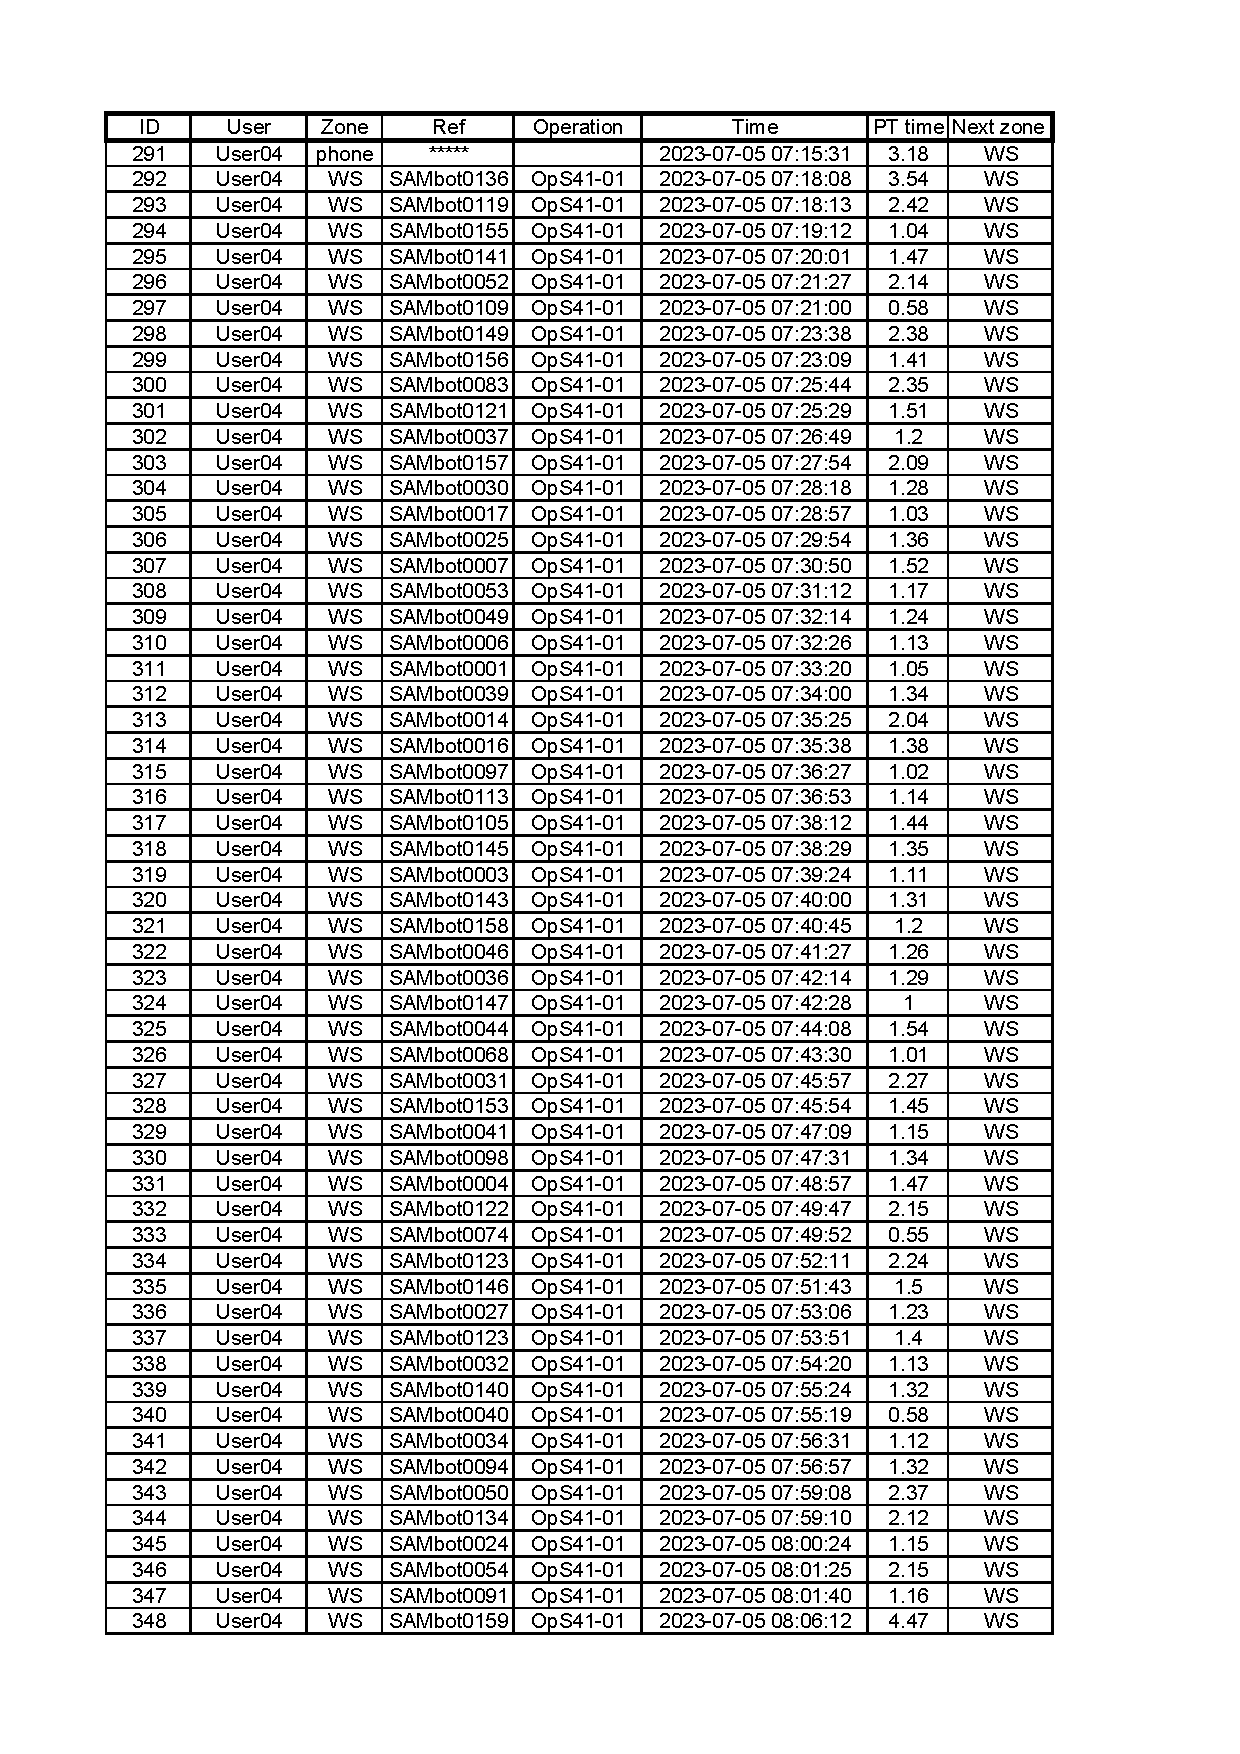
\includepdf[pages=-]{data.pdf}

% \begin{thebibliography}{00}
% \expandafter\ifx\csname url\endcsname\relax
%   \def\url#1{\texttt{#1}}\fi
% \expandafter\ifx\csname urlprefix\endcsname\relax\def\urlprefix{URL }\fi
% \expandafter\ifx\csname href\endcsname\relax
%   \def\href#1#2{#2} \def\path#1{#1}\fi
  
% \bibitem{Acar2018Creativity}
% Acar, O., Tarakci, M., \& Knippenberg, D. (2018). Creativity and Innovation Under Constraints: A Cross-Disciplinary Integrative Review. Journal of Management, 45, 121 - 96.

% % Generating creative ideas and turning them into innovations is key for competitive advantage. However, endeavors toward creativity and innovation are bounded by constraints such as rules and regulations, deadlines, and scarce resources. The effect of constraints on creativity and innovation has attracted substantial interest across the fields of strategic management, entrepreneurship, industrial organization, technology and operations management, organizational behavior, and marketing. Research in these fields has focused on various constraints that trigger distinct mediating mechanisms but is fragmented and yields conflicting findings. We develop a taxonomy of constraints and mediating mechanisms and provide an integrative synthesis that explains how constraints affect creativity and innovation. Our review thus facilitates cross-disciplinary learning and sets the stage for further theoretical development.



% \bibitem{Abii2013Effects}
% Abii, F., Ogula, D., \& Rose, J. (2013). Effects of Individual and Organizational Factors on the Turnover Intentions of Information Technology Professionals. The International Journal of Management, 30, 740.
% % High employee turnover is a problem that organizations cannot ignore because of the financial burden, negative impact on employee morale, and employee relationships, and adverse impact on the quality of services and products that organizations deliver to customers. The apparent high employee turnover rates in the Information Technology (IT) industry suggests that the factors influencing turnover in the industry may not be well understood. This quantitative study examined the organizational and individual  factors that influence IT employees’ decisions to leave an organization. The results of the study indicate that employee compensation and workplace relationships are factors

% \bibitem{Jamal2019Work}
% Jamal, A. (2019). Work Turnover and Its Impact on the Quality of Productivity in the Industrial Sector. Research in World Economy, 10, 65.

% % The aim of this study was to identify the effect of high turnover on quality of productivity in the industrial sector, and to propose appropriate solutions to reduce the reasons for leaving work. The motivation to carry out this study, the spread of the turnover phenomenon leading to dysfunction is in the interest of the organization, and has a direct impact on the decline in the quality of productivity of the organization, so was applied to the industrial sector to know and measure this impact. The methodology used in this study is the descriptive and analytical approach and the case study methodology. The results of the study show that there is a relationship of statistical significance between the average level of performance of the employee and the level of total productivity in the organization. And that there is a middle relationship between job stability and employee performance level, and that there is a negative relationship between the turnover rate and quality of productivity in the industrial sector. The study recommends that employers try to retain existing workers and provide appropriate incentives for them to reduce the rate of turnover in institutions, because turnover is a cost to institutions that can be eliminated by retaining staff and institutions should improve financial and non-financial compensation in proportion to the circumstances And staff needs to ensure job stability and ensure quality of productivity.
% that influence turnover
% \end{thebibliography}

\end{document}

